\documentclass[12pt]{article}
\usepackage{inputenc}
\usepackage{graphicx}
\usepackage{tabularx}
\usepackage{hyperref}

%%%%%%%%%%%%%%%%
% Impostazioni %
%%%%%%%%%%%%%%%%

\hypersetup{
    colorlinks=true,
    linkcolor=blue,
    filecolor=magenta,
    urlcolor=cyan,
    pdftitle={Database Concerti, Michael Guidelli},
    pdfpagemode=FullScreen,
}

\date{}

\begin{document}

%%%%%%%%%%
% Titolo %
%%%%%%%%%%

\maketitle
\null \null \null \null \null \null
{\centering
    \huge\bfseries Database Concerti \\
    \Large\normalfont Michael Guidelli  \\
}

\clearpage

%%%%%%%%%%%%%%%%%%%%%
% Traccia esercizio %
%%%%%%%%%%%%%%%%%%%%%

\section*{Traccia esercizio}

\noindent
\textbf{ITI “G. Ferraris” - Verifica Scritta di informatica Classe VBSE – Prof. Andrea Arcella} \newline

\noindent
Si vuole progettare la base di dati di un’applicazione relativa ad un programma di concerti,
secondo le seguenti specifiche.

\begin{itemize}
    \item Ogni concerto ha un codice, un titolo e una descrizione, ed è composto da una sequenza (ordinata) di pezzi musicali.
    
    \item Ogni pezzo ha un codice, un titolo e un autore (con codice e nome); uno stesso pezzo può essere rappresentato in diversi concerti.
    
    \item Ogni concerto è eseguito da un gruppo; ogni gruppo ha un nome, e un insieme di componenti.
    
    \item Ogni componente ha una matricola (univoca nell’ambito della base di dati), nome e cognome, può partecipare a più gruppi, e suona uno o più strumenti, gli stessi in ciascuno dei gruppi.
    
    \item Ogni concerto è tenuto più volte, in date diverse, ma sempre nella stessa sala.
    
    \item Ogni sala ha un codice, un nome e una capienza.
\end{itemize}

\noindent
Dopo eventuali ipotesi aggiuntive

\begin{enumerate}
    \item Effettuare la progettazione concettuale dell’applicazione, producendo il relativo schema Entità-Relazione.
    
    \item Effettuare la progettazione logica dell’applicazione, producendo il relativo schema delle tabelle e avendo cura di specificare il tipo di dati per ogni campo della tabella
    
\end{enumerate}

\clearpage 

%%%%%%%%%%%%%%%%%%%%%%%%%%%%%%%%
% Impostazioni indice e figure %
%%%%%%%%%%%%%%%%%%%%%%%%%%%%%%%%%

\renewcommand{\contentsname}{Indice \label{indice}}
\tableofcontents

\renewcommand{\listfigurename}{Lista delle figure}
\listoffigures

\renewcommand{\listtablename}{Liste Attributi}
\listoftables

\clearpage

%%%%%%%%%%%
% Ipotesi %
%%%%%%%%%%%

\section{Ipotesi}

\begin{enumerate}
    \item Ipotizzo che un pezzo possa essere scritto da più autori, quindi la cardinalità  dell'associazione \textbf{Scrive} sarà \textbf{N} a \textbf{N}.
\end{enumerate}

%%%%%%%%%%%%%%%%%%%%%%%%%%%%%%%%%%%
% Scelta attributo identificativo %
%%%%%%%%%%%%%%%%%%%%%%%%%%%%%%%%%%%

\section{Criterio scelta attributi identificativi}

\noindent
Nella scelta degli attributi ho potuto constatare che tutte le entità eccetto l'entità componente, non hanno un attributo identificativo indicato dal testo, quindi ho creato degli attributi identificativi formati da numeri/lettere indicati con: id più il nome dell'entità. Nel caso dell'entità componente l'attributo matricola ha le caratteristiche per essere l'attributo identificativo.

\clearpage

%%%%%%%%%%%%%%
% Modello ER %
%%%%%%%%%%%%%%

\section{Modello ER}
\begin{figure}[h!]
    \centering
    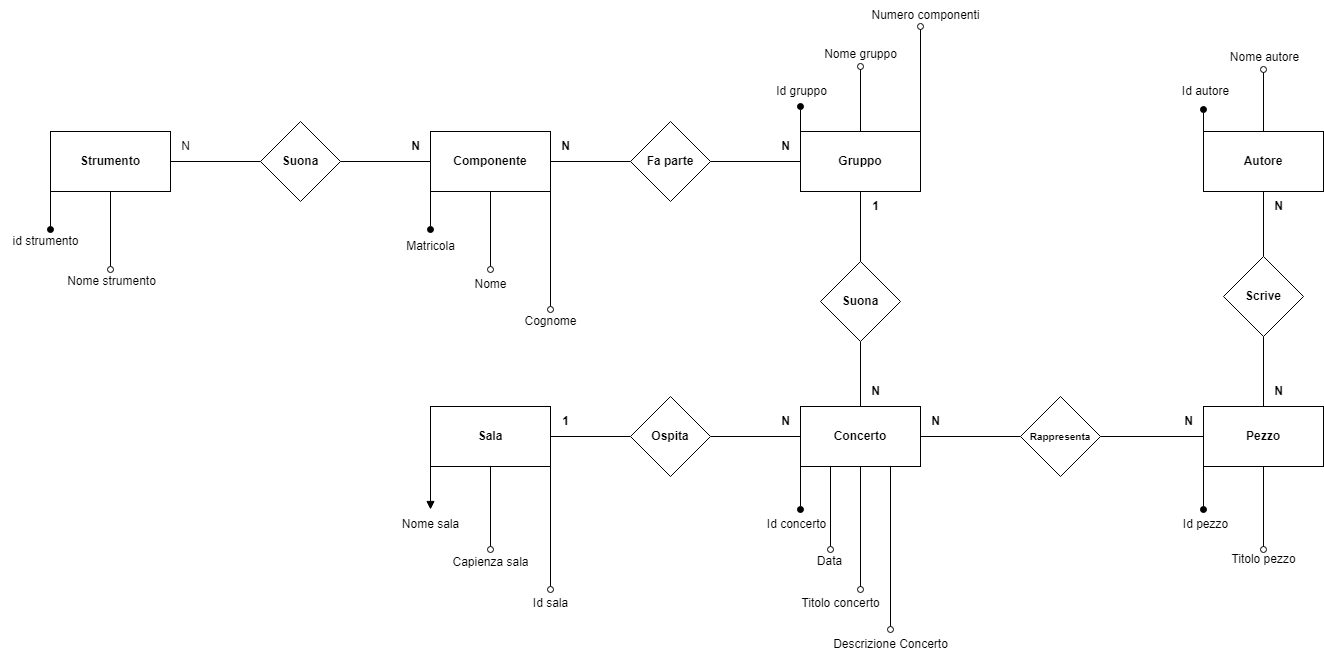
\includegraphics[width=16cm]{modello_er_concerto.png}
    \caption{Rappresentazione modello ER}
    \label{fig: modello er concerto}
\end{figure}

%%%%%%%%%%%%%%%
% Cardinalità %
%%%%%%%%%%%%%%%

\subsection{Cardinalità}

\noindent
Cardinalità delle associazioni:

\begin{itemize}
    \item \textbf{Rappresenta}: In questo caso la cardinalità è \textbf{N} a \textbf{N} perché ciascun singolo concerto può rappresentare uno o più pezzi e ciascun singolo pezzo può essere rappresentato da più concerti.
    
    \item \textbf{Scrive}: In questo caso la cardinalità è \textbf{N} a \textbf{N} perché ciascun singolo autore può scrivere uno o più pezzi e ciascun singolo pezzo può essere scritto da più autori.
    
    \item \textbf{Ospita}: In questo caso la cardinalità è \textbf{1} a \textbf{N} perché ciascun singolo concerto può essere ospitato da una sala e ciascuna singola sala può ospitare più concerti in date diverse.
    
    \item \textbf{Suona}: In questo caso la cardinalità è \textbf{1} a \textbf{N} perché ciascun singolo concerto può essere suonato da un gruppo e ciascun singolo gruppo può suonare più concerti.
    
    \item \textbf{Fa parte}: In questo caso la cardinalità è \textbf{N} a \textbf{N} perché ciascun singolo componente può far parte di uno o più gruppi e a ciascun singolo gruppo fanno parte più componenti.
    
    \item \textbf{Suona}: In questo caso la cardinalità è \textbf{N} a \textbf{N} perché ciascun singolo componente suona uno o più strumenti e ciascun singolo strumento può essere suonato da più componenti.
\end{itemize} 

\clearpage

%%%%%%%%%%%%%%%%%%%%%%%%%
% Liste degli attributi %
%%%%%%%%%%%%%%%%%%%%%%%%%

\begin{center}
    \section{Liste degli attributi}
\end{center}

% Entità concerto %

\subsection*{Lista attributi Concerto}
\begin{table}[h!]
    \centering
    \begin{tabular}{|c|c|c|c|}
        \hline
         Nome attributo & Significato & Tipo di dato & Vincolo  \\
        \hline
        Id concerto & Attributo identificativo & Varchar & Max 255 caratteri  \\
        \hline
        Data & Data del concerto & Date & \\
        \hline 
        Titolo & Titolo del concerto & Varchar & Max 255 caratteri \\ 
        \hline
        Descrizione & Descrizione del concerto & Text & Max 300 caratteri \\
        \hline
    \end{tabular}
    \caption{Lista Concerto}
    \label{tab: tabella entità concerto}
\end{table}

% Entità pezzo %

\subsection*{Lista attributi Pezzo}
\begin{table}[h!]
    \centering
    \begin{tabular}{|c|c|c|c|}
        \hline
        Nome attributo & Significato & Tipo di dato & Vincolo  \\
        \hline 
        Id pezzo & Attributo identificativo & Varchar & Max 255 caratteri \\
        \hline
        Titolo & Titolo del pezzo & Varchar & Max 255 caratteri \\
        \hline
    \end{tabular}
    \caption{Lista Pezzo}
    \label{tab: tabella entità pezzo}
\end{table}

% Entità autore %

\subsection*{Lista attributi Autore}
\begin{table}[h!]
    \centering
    \begin{tabular}{|c|c|c|c|}
        \hline
        Nome attributo & Significato & Tipo di dato & Vincolo \\
        \hline 
        Id autore & Attributo identificativo & Varchar & Max 255 caratteri \\
        \hline
        Nome & Nome autore & Varchar & Max 255 caratteri \\ 
        \hline
    \end{tabular}
    \caption{Lista Autore}
    \label{tab: tabella entità autore}
\end{table}

\clearpage

% Entità sala %

\subsection*{Lista attributi Sala}
\begin{table}[h!]
    \centering
    \begin{tabular}{|c|c|c|c|}
        \hline
        Nome attributo & Significato & Tipo di dato & Vincolo \\
        \hline
        Id sala & Attributo identificativo & varchar & Max 255 caratteri \\
        \hline
        Nome & Nome della sala & Varchar & Max 255 caratteri \\
        \hline
        Capienza & Capienza della sala & Int & Max 4 cifre \\
        \hline
    \end{tabular}
    \caption{Lista Sala}
    \label{tab: tabella entità sala}
\end{table}

% Entità gruppo %

\subsection*{Lista attributi Gruppo}
\begin{table}[h!]
    \centering
    \begin{tabular}{|c|c|c|c|}
        \hline
        Nome attributo & Significato & Tipo di dato & Vincolo \\
        \hline
        Id gruppo & Attributo identificativo & Varchar & Max 255 caratteri \\
        \hline
        Nome & Nome del gruppo & Varchar & Max 255 caratteri \\
        \hline
        Componenti & Numero componenti & Int & Max 3 cifre \\
        \hline
    \end{tabular}
    \caption{Lista Gruppo}
    \label{tab: tabella entità gruppo}
\end{table}

% Entità componente % 

\subsection*{Lista attributi Componente}
\begin{table}[h!]
    \centering
    \begin{tabular}{|c|c|c|c|}
        \hline
        Nome attributo & Significato & Tipo di dato & Vincolo \\
        \hline
         Matricola & Attributo identificativo & Varchar & Max 255 caratteri \\
        \hline
        Nome & Nome componente & Varchar & Max 255 caratteri \\
        \hline
        Cognome & Cognome componente & Varchar & Max 255 caratteri \\
        \hline
    \end{tabular}
    \caption{Lista Componente}
    \label{tab: tabella entità componente}
\end{table}

\clearpage

% Entità strumento % 

\subsection*{Lista attributi Strumento}

\begin{table}[h!]
    \centering
    \begin{tabular}{|c|c|c|c|}
        \hline
        Nome attributo & Significato & Tipo di dato & Vincolo \\
        \hline
        Id strumento & Attributo identificativo & Varchar & Max 255 caratteri \\
        \hline
        Nome & Nome strumento & Varchar & Max 255 caratteri \\
        \hline
    \end{tabular}
    \caption{Lista Strumento}
    \label{tab: tabella entità strumento}
\end{table}

\end{document}